\newpage
\section{Analysis}

Once the code has been completed and the functionality has been verified (See section xxx for verification) we have automated the process to run the application for every possible input size $1 \leq size \leq 128$ and collect all the timing information to conduct performance analysis and get more insight into the application's behavior under different input sizes.

Figure~\ref{fig:perf_plot} shows execution time for different valid input sizes for different configurations. To facilitate the analysis a more elaborate plot with speedups has been made in Figure~\ref{fig:speedup_plot} which shows speedups for different valid input sizes for DSP+NEON and NEON only configurations. This figure shows us a number of useful insights:
\begin{itemize}
\item{NEON+DSP shows slowdown for $size < 60 + \epsilon$}
\item{NEON only configuration performs better for $size < 90 + \epsilon$}
\item{NEON+DSP configuration is best for $size >90 + \epsilon$}
\item{NEON only configuration performs better than serial execution $ \forall size$}

\end{itemize}



\begin{figure}[h!]
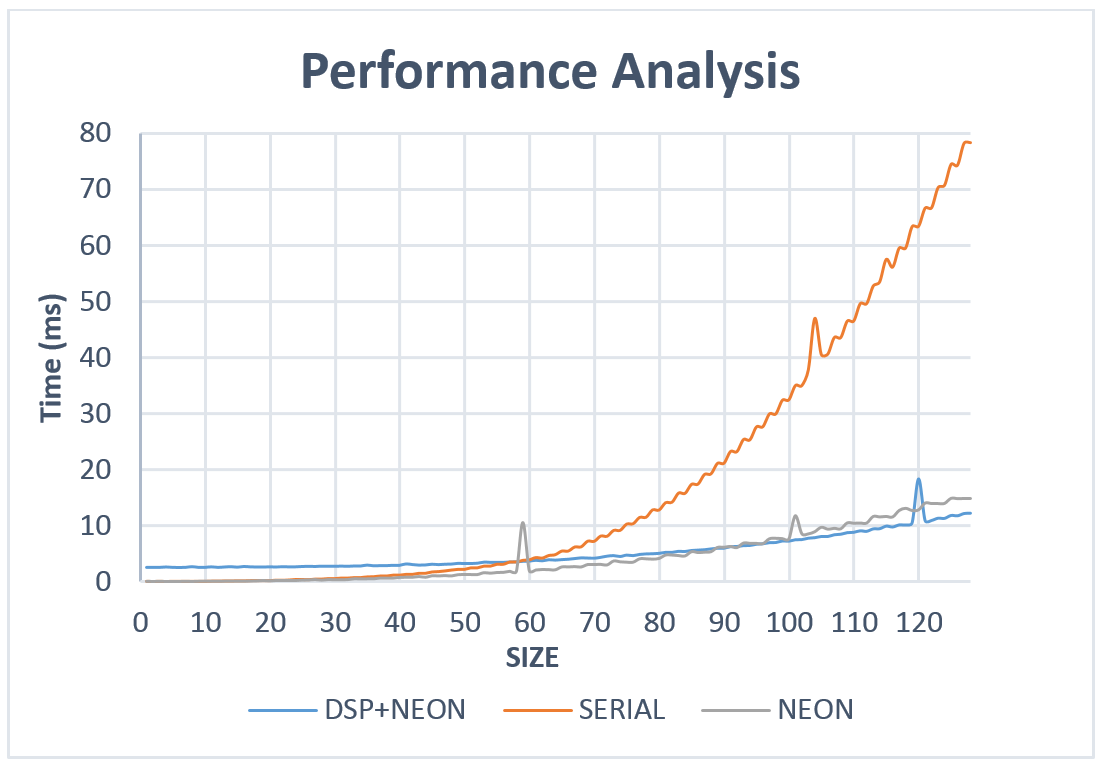
\includegraphics[width=\textwidth]{analysis/perf_plot}
\caption{Performance Analysis plot: Execution times as a function of input size for different configurations}
\label{fig:perf_plot}
\end{figure}


\begin{figure}[h!]
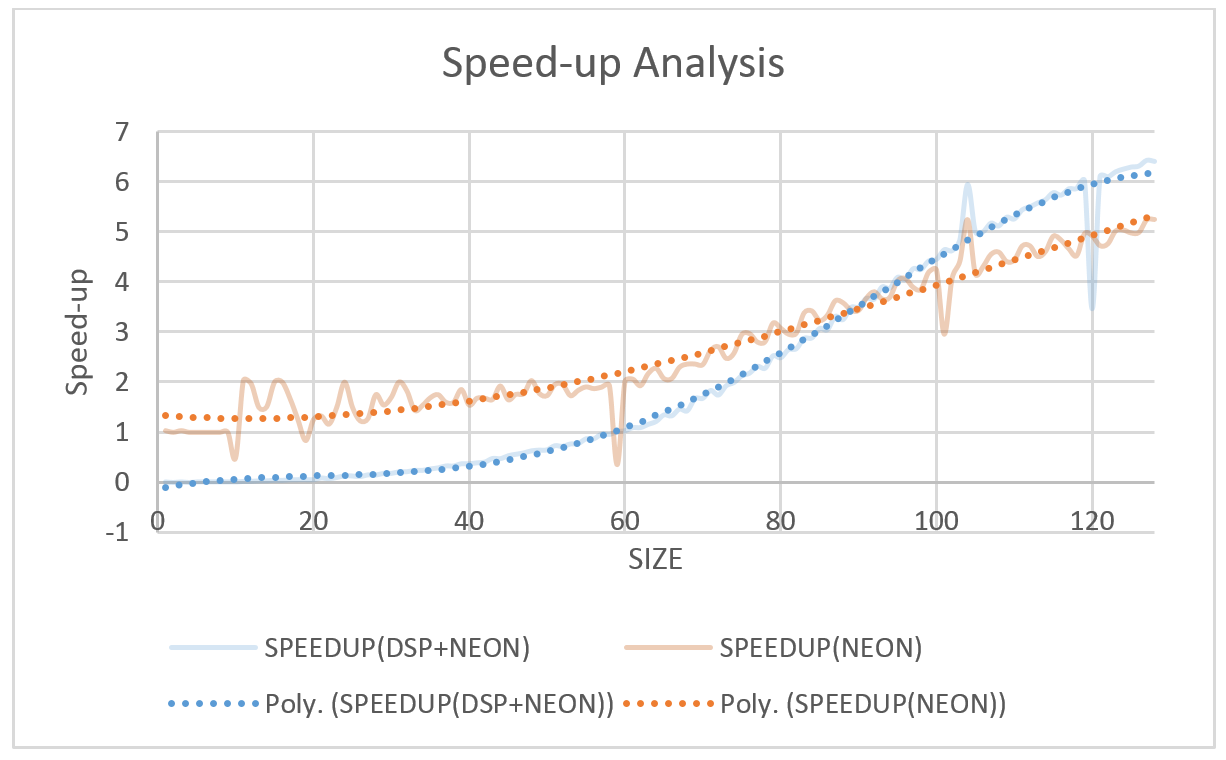
\includegraphics[width=\textwidth]{analysis/speedup_plot}
\caption{Speed-up plot: Achievable speed-up as a function of input size for different configurations}
\label{fig:speedup_plot}
\end{figure}

